\chapter{Progress}

Budd's sliding theory describes stress propagation through flowing ice over undulating bedrock. The stress field propagates upward at an angle, creating surface waves that are phase-shifted by approximately $\pi/2$ relative to bedrock features, in Budd's words: ``the maximum shear stress occurs at the tops of the waves and the minimum in the troughs''\cite{Budd_1970}. To test this theory, my ISSM simulation uses a flowband model in a 27 km domain (triangular elements sized at 0.8 km), 2.7 km mean ice thickness, bedrock at 1 km elevation with -0.1 radian slope, and cosine undulations (9.72 km wavelength, 0.054 km amplitude). I chose these parameters based on the most ideal transference conditions explained in \cite{Budd_1970}. I ran a 300-year Full-Stokes transient simulation with 1-year time steps. The results show that the relationship between surface and bedrock profiles does not exhibit the expected $\pi/2$ phase shift but instead shows a shift of -0.04$\pi$ radians, which corresponds to a spatial shift of -0.200 km (see Figures \ref{fig:direct} and \ref{fig:xcorr}). This effect is directly attributable to Budd's shear stress function (see Figure \ref{fig:friction}). The discrepancy between my results and Budd's theory could very well be due to my simulation not yet reaching steady state. Given my recent acquisition of ISSM skills, I have not yet had the opportunity to utilize the NCI supercomputing platform Gadi, but I am in the process of transitioning from local simulations to this more powerful to achieve the extended run times necessary for steady-state analysis.

\begin{figure}[H]
    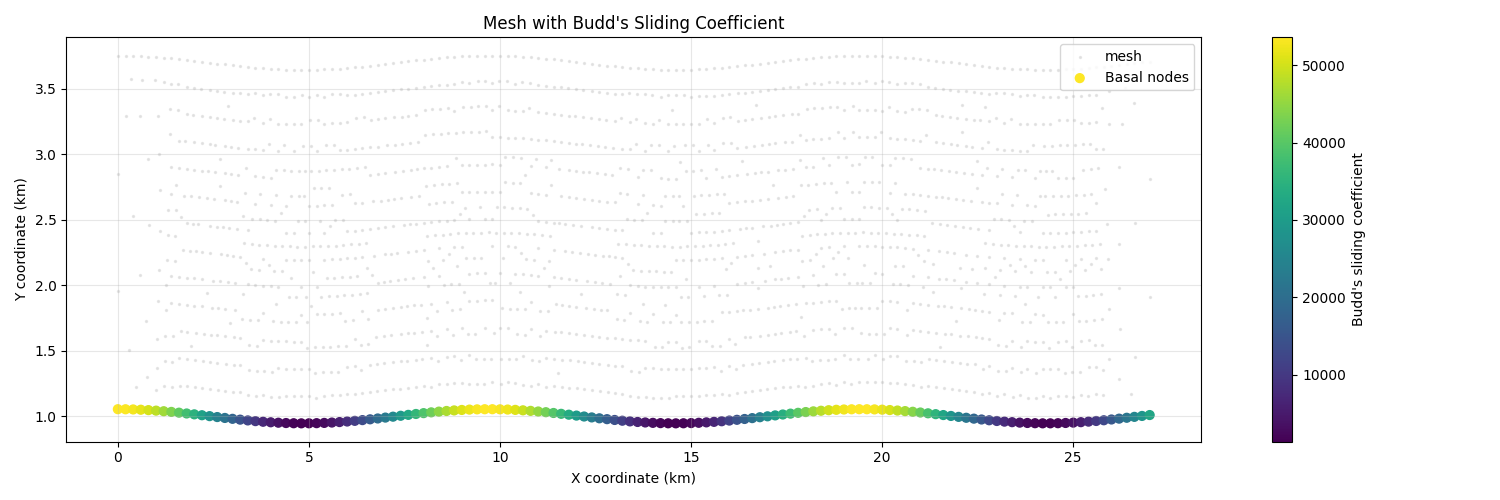
\includegraphics[scale=0.5]{basal_friction.png}
    \caption{Slope parallel visualisation of the computational mesh with basal nodes highlighted. The gray dotted lines represent the complete finite element mesh with multiple vertical layers conforming to the undulating geometry. Basal nodes (purple to yellow) follow the periodic undulated bed topography with wavelength 9.72 km and amplitude 0.054 km. The colour gradient along the basal nodes displays the imposed variations in basal shear stress corresponding to Budd's sliding law, with lighter colours indicating regions of higher basal drag. Note that maximum basal drag occurs near the peaks of the bedrock undulations, consistent with the expected shear stress pattern in the sliding theory. The 27 km domain contains approximately three complete undulation cycles.}
    \label{fig:friction}
\end{figure}

\begin{figure}
    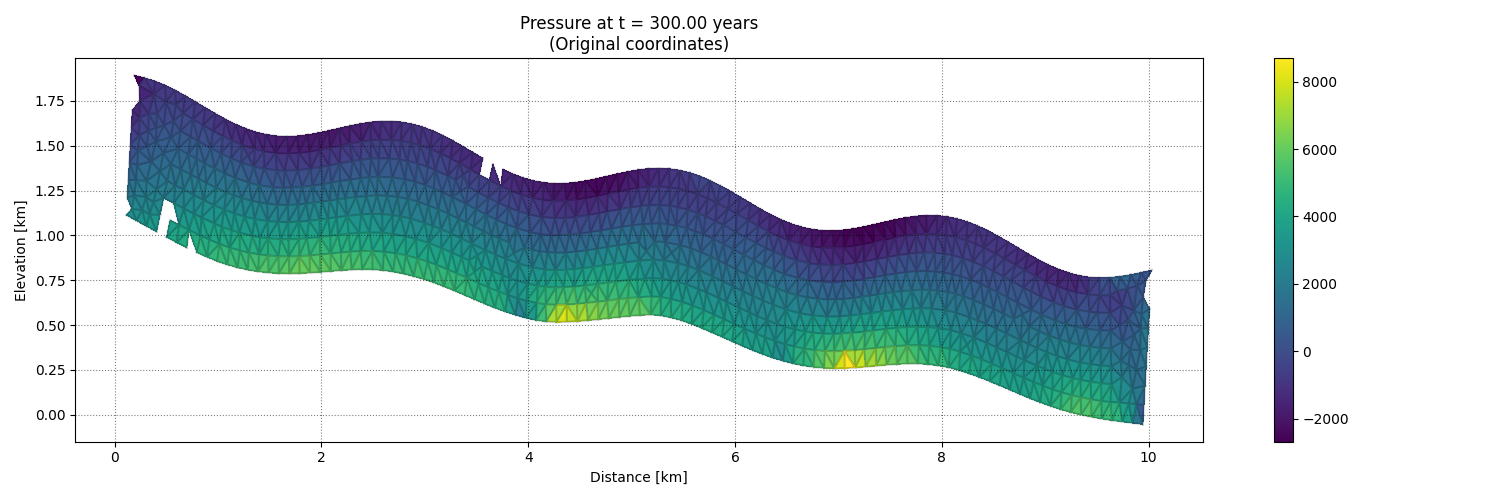
\includegraphics[scale=0.45]{Pressure_300yrs_xz.png}
    \caption{Pressure field distribution at t = 300.00 years shown in original coordinates. The color scale reveals the spatial pressure variations throughout the ice body, with higher pressures (yellow) concentrated at the base and particularly near bedrock peaks. The triangular mesh elements display the finite element discretisation used for solving the Full-Stokes equations. The overall pressure gradient follows ice thickness with maximum values at the base with a visible influence of bedrock undulations on the pressure field. The downward-sloping ice surface reflects the -0.1 radian background slope condition, while subtle surface undulations are apparent in response to the bed topography. This visualization captures the result after 300 years of transient simulation, providing insight into the stress propagation patterns described in Budd's sliding theory.}
    \label{fig:Pressure}
\end{figure}
% Note: The white gaps visible within the mesh represent masked areas excluded from visualization processing, not physical features or data gaps in the original simulation.

\begin{figure}
    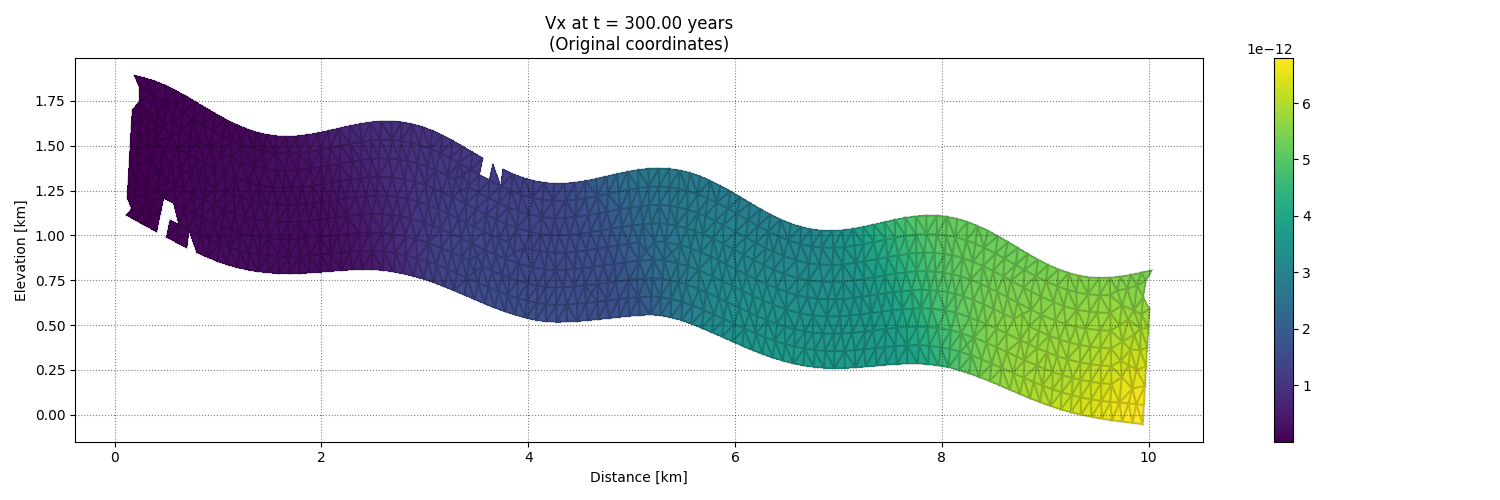
\includegraphics[scale=0.45]{Vx_300yrs_xz.png}
    \caption{
    Horizontal velocity field ($V_x$) at t = 300.00 years displayed in original coordinates. The color scale indicates velocity magnitudes ranging from 0 to 0.0147 km per year with flow direction from left to right. The velocity pattern shows clear acceleration as the ice flows downslope, with highest velocities (yellow) occurring near the terminus region. The fixed upstream boundary condition constrains flow at the inlet, while the progressive acceleration downstream results from gravitational forcing along the -0.1 radian sloped bed. Note the visible influence of the bedrock undulations on the velocity field, particularly near the base. The contrast between slow-moving upper ice (purple) and faster basal ice in the terminal region demonstrates the development of vertical velocity gradients.}
    \label{fig:Vx}
\end{figure}


\begin{figure}
    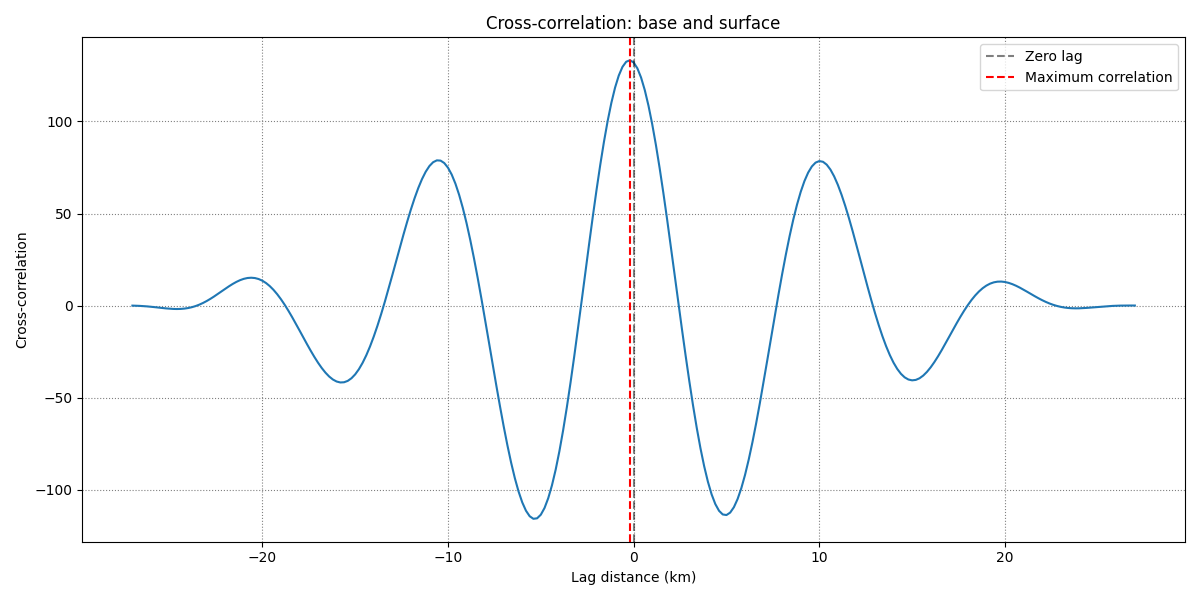
\includegraphics[scale=0.5]{xcorr.png}
    \caption{Cross-correlation between the bedrock elevation and surface slope signals across spatial lags. The blue curve shows normalized correlation coefficients as a function of lag distance. The maximum correlation (red dashed line) occurs at a lag distance of -0.2 km, which translates to a phase shift of -0.04$\pi$ radians (-7.4 degrees). This observed phase shift significantly deviates from Budd's theoretical prediction of $\pi/2$ (90 degrees), suggesting that in this simulation at t = 300 years, the relationship between bedrock topography and surface features differs from theory. The zero lag position (black dashed line) represents perfect spatial alignment. The periodic nature of the cross-correlation function reflects the underlying 9.72 km wavelength of the bedrock undulations, with correlation peaks appearing at approximately 10 km intervals.}
    \label{fig:xcorr}
\end{figure}

\begin{figure}
    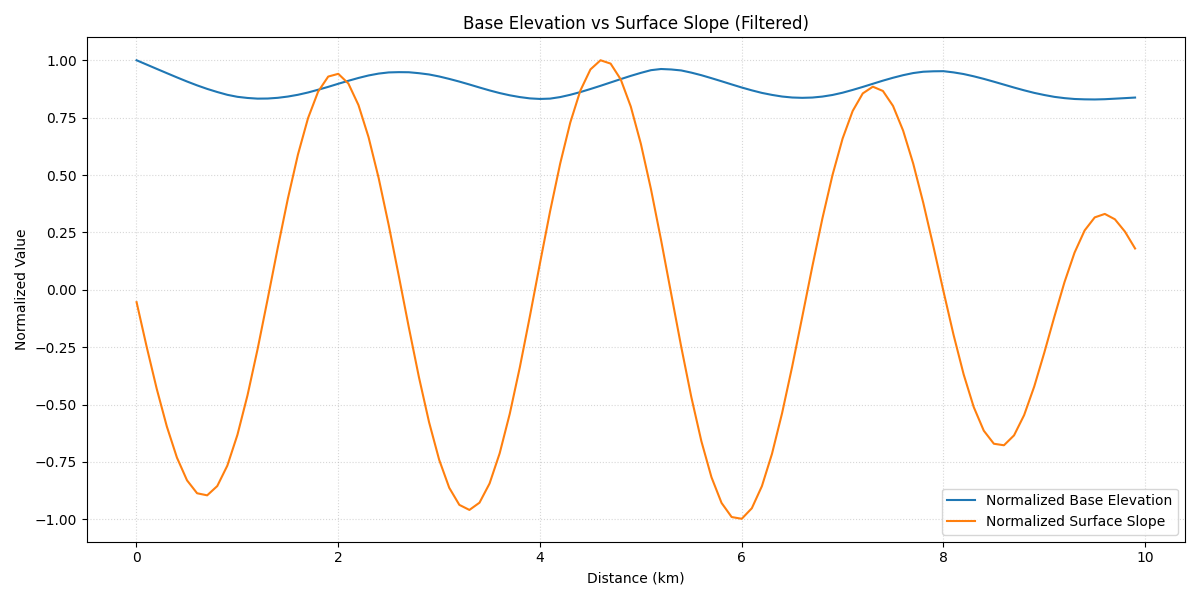
\includegraphics[scale=0.5]{direct.png}
    \caption{Direct comparison between bedrock topography (black) and ice surface elevation (blue) with mean elevations removed to highlight the undulation patterns. Both profiles are plotted in slope-parallel coordinates along the 27 km domain. The surface undulations exhibit a visible phase shift relative to the bedrock features, though this shift is noticeably less than the theoretical $\pi/2$ predicted by Budd's sliding theory. The surface amplitude appears damped compared to the bed amplitude, particularly evident in the central wavelengths. However, boundary effects near $x = 0$ and $x = 27$ km complicate the interpretation, as the amplitude damping and phase relationships may be influenced by the finite domain and boundary conditions. This comparison at t = 300 years reveals a complex and still-evolving relationship between bed topography and surface expression, with the phase relationship varying slightly across the domain. The dominant wavelength of approximately 9.72 km is preserved in both signals, indicating effective stress transmission through the 2.7 km ice thickness despite the reduced phase shift.}
    \label{fig:direct}
\end{figure}

\begin{figure}
    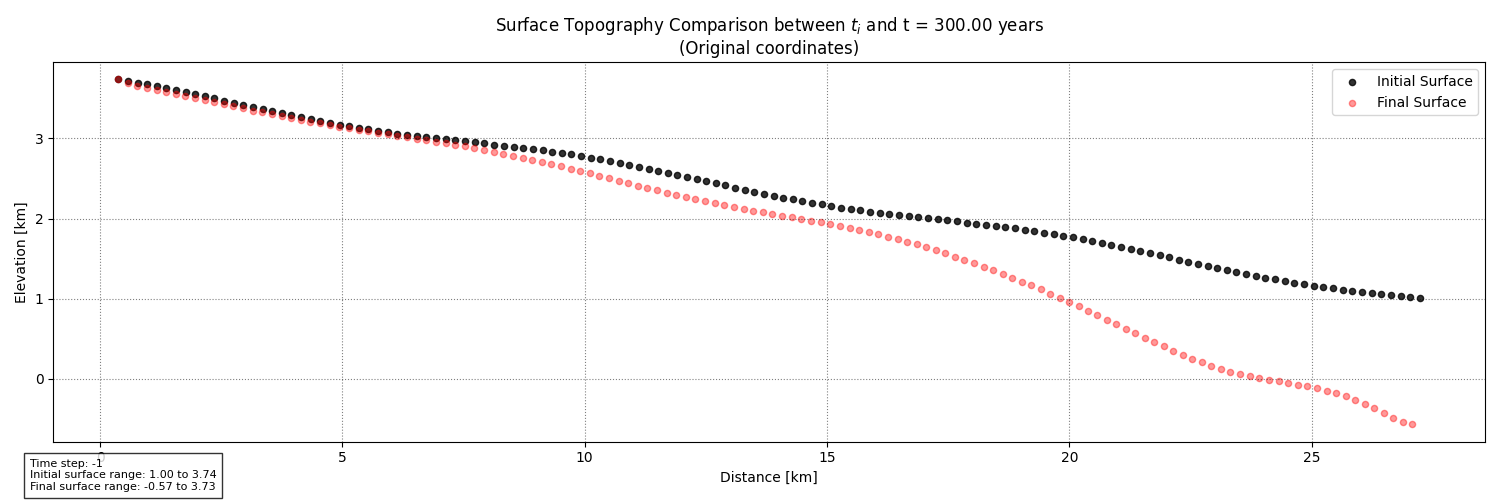
\includegraphics[scale=0.45]{surfaces_comparison.png}
    \caption{Evolution of ice surface topography from initial condition (black) to final state at t = 300.00 years (red) displayed in original coordinates. The simulation shows significant ice thinning and terminus retreat, with the final surface elevation ranging from -0.57 to 3.73 km compared to the initial range of 1.00 to 3.74 km. The final surface exhibits a steeper overall slope, particularly in the lower half of the domain ($x > 15$ km), indicating a dynamic response to the applied flow conditions. Surface undulations have developed in the final state, though these are subtle relative to the overall elevation change. The preservation of similar elevation at the upper boundary ($x = 0$ km) reflects the fixed inflow boundary condition, while the downstream region shows maximum adjustment. This 300-year evolution demonstrates that the ice mass is still adapting to the prescribed basal conditions and has not yet reached a steady state, which may explain the discrepancy between the observed phase shift and Budd's theoretical prediction.}
    \label{fig:surfaces}
\end{figure}

